
\documentclass[fleqn,addpoints]{exam}

\usepackage{graphicx}
\usepackage{float}
\usepackage{amsmath}
\usepackage{cancel}
\usepackage{polynom}
\usepackage{caption}

\printanswers

\ifprintanswers 
\usepackage{2in1, lscape} 
\fi

\title{Math 115 \\ Homework 16}
\date{\today}

\begin{document}

\maketitle

% \begin{figure}[H]
%   \centering
%   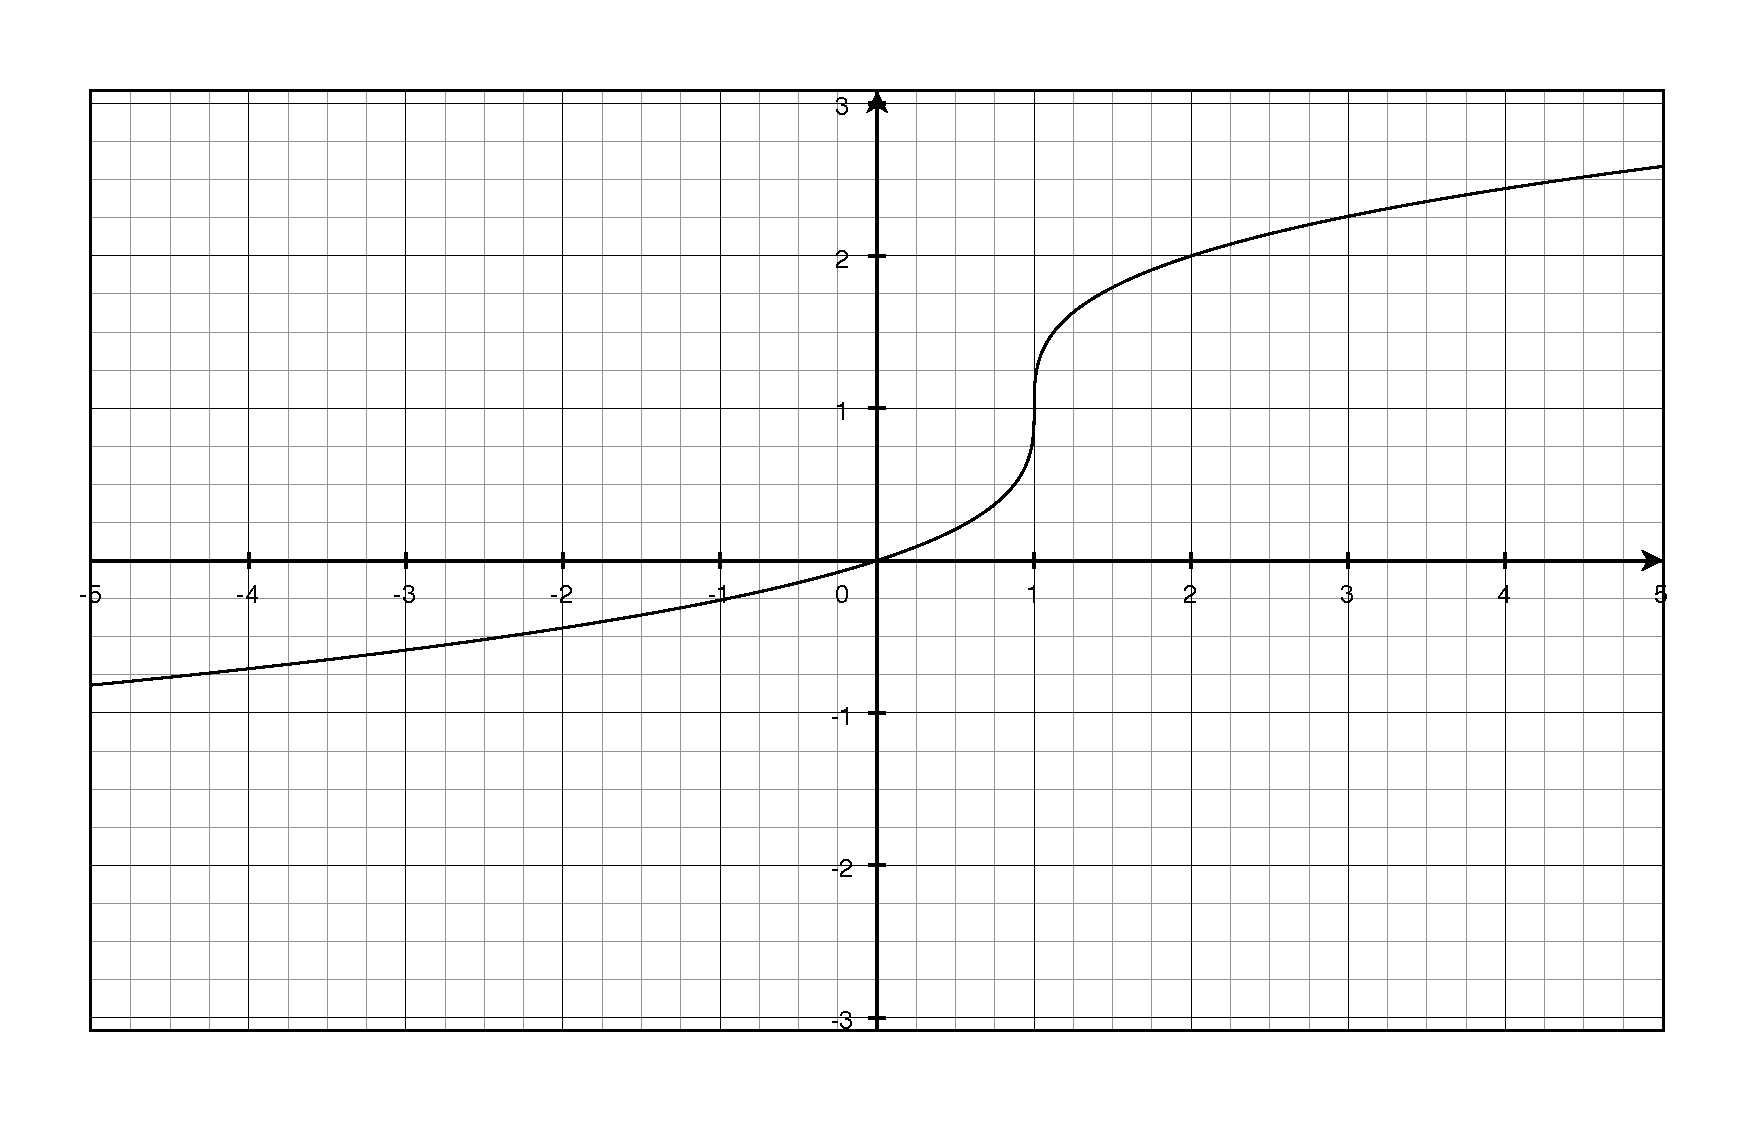
\includegraphics[scale=.3]{question7.eps}
%   \caption*{Question 7}
% \end{figure}

\section{Homework}

\begin{itemize}
  \item Read Section 3.3
  \item pp 315-316: 1-5, 10-11, 25-30, 39-42, 50-54, 60-62, 65, 67, 71, 78, 85, 87-91
\end{itemize}

\ifprintanswers
\begin{description}

\item[1]
\[
  \log_3 7 = 1.771
\]

\item[2]
\[
  \log_7 4 = 0.712
\]

\item[3]
\[
  \log_{1/2} 4 = -2
\]

\item[4]
\[
  \log_{1/4} 5 = -1.161
\]

\item[5]
\[
  \log_9 0.4 = -0.417
\]

\item[10]
\begin{description}

\item[a]
\[
  \log_3 x = \frac{\log x}{\log 3}
\]

\item[b]
\[
  \log_3 x = \frac{\ln x}{\ln 3}
\]

\end{description}

\item[11]
\begin{description}

\item[a]
\[
  \log_{1/5} x = \frac{\log x}{\log 1/5}
\]

\item[b]
\[
  \log_{1/5} x = \frac{\ln x}{\ln 1/5}
\]

\end{description}

\item[25]
\[
  \log_{10} \frac{5}{x} = \log_{10} 5 - \log_{10} x
\]

\item[26]
\[
  \log_{10} \frac{y}{2} = \log_{10} y - \log_{10} 2 
\]

\item[27]
\[
  \log_8 x^4 = 4 \log_8 x
\]

\item[28]
\[
  \log_6 z^{-3} = -3 \log_6 z
\]

\item[29]
\[
  \ln \sqrt{z} = \ln z^{1/2} = \frac{1}{2} \ln z
\]

\item[30]
\[
  \ln \sqrt[3]{t} = \ln t^{1/3} = \frac{1}{3} \ln t
\]

\item[39]
\begin{align*}
  \ln \frac{x^4 \sqrt{y}} {z^5} &= \ln x^4y^{1/2} - \ln z^5 \\
   &= \ln x^4 + \ln y^{1/2} - 5 \ln z \\
   &= 4 \ln x + \frac{1}{2} \ln y - 5 \ln z
\end{align*}

\item[40]
\begin{align*}
  \ln \sqrt{x^2(x+2)} &= \ln (x^2(x+2))^{1/2} \\ 
  &= \frac{1}{2} \ln (x^2(x+2)) \\ 
  &= \frac{1}{2} (\ln x^2 + \ln(x+2) ) \\ 
  &= \frac{1}{2} (2 \ln x + \ln(x+2) ) \\ 
  &= \ln x + \frac{\ln(x+2)}{2} \\ 
\end{align*}

\item[41]
\begin{align*}
  \log_b \frac{x^2}{y^2z^3} &= \log_b x^2 - \log_b y^2z^3 \\
  &= 2 \log_b x - (\log_b y^2 + \log_b z^3) \\
  &= 2 \log_b x - 2 \log_b y - 3 \log_b z \\
\end{align*}

\item[42]
\begin{align*}
  \log_b \frac{\sqrt{x} y^4}{z^4} &= \log_b \frac{x^{1/2} y^4}{z^4} \\
  &= \log_b x^{1/2} y^4 - \log_b z^4 \\
  &= \log_b x^{1/2} + \log_b y^4 - \log_b z^4 \\
  &= \frac{1}{2} \log_b x + 4 \log_b y - 4 \log_b z \\
\end{align*}

\item[50]
\[
  \frac{2}{3} \log_7(z-2) = \log_7(z-2)^{2/3}
\]

\item[51]
\[
  \ln x - 3 \ln(x+1) =   \ln x - \ln(x+1)^3 = \ln \frac{x}{(x+1)^3}
\]

\item[52]
\[
  2 \ln 8 + 5 \ln z = \ln 8^2 + \ln z^5 = \ln 64z^5
\]

\item[53]
\[ 
\ln(x-2) - \ln(x+2) = \ln \frac{x-2}{x+2}
\]

\item[54]
\begin{align*}
  3 \ln x + & 4 \ln y - 4 \ln z \\
  &= \ln x^3 + \ln y^4 - \ln z^4 \\
  &= \ln x^3y^4 - \ln z^4 \\
  &= \ln \frac{x^3y^4}{z^4} \\
\end{align*}

\item[60]
\begin{align*}
  \frac{1}{2} [ \ln(x+1) + & 2 \ln (x-1) ] + 6 \ln x \\
  &= \frac{1}{2} \ln(x+1) + \ln(x-1) + \ln x^6 \\
  &= \ln(x+1)^{1/2} + \ln(x-1) + \ln x^6 \\
  &= \ln \left[ x^6(x-1)(x+1)^{1/2} \right] \\
\end{align*}

\item[61]
\begin{align*}
  2 \ln 3 - \frac{1}{2} \ln(x^2 + 1) &= \ln 3^2 - \ln (x^2+1)^{1/2} \\
  &= \ln 9 - \ln (x^2+1)^{1/2} \\
  &= \ln \left[ \frac{9}{(x^2+1)^{1/2}} \right] \\
\end{align*}

\item[62]
\begin{align*}
  \frac{3}{2} \ln 5t^6 - \frac{3}{4} \ln t^4 &= \ln (5t^6)^{3/2} - \ln t^3 \\
  &= \ln 5^{3/2}t^9 - \ln t^3 \\
  &= \ln \frac{5^{3/2}t^9}{t^3} \\
  &= \ln 5^{3/2}t^6 \\
\end{align*}

\item[65]
\[ \log_3 9 = \log_3 3^2 = 2\]

\item[67]
\[
  \log_4 16^{1.2} = 1.2 \log_4 16 = 1.2 \cdot 2 = 2.4
\]

\item[71]
\[
  \log_5 75 - \log_5 3 = \log_5 \frac{75}{3} = \log_5 25 = 2
\]

\item[78]
\[
  \ln \sqrt[4]{e^3} = \ln e^{3/4} = \frac{3}{4}
\]

\item[85]
\begin{description}

\item[a] $f(0) = 90$

\item[b] $f(6) = 77$

\item[c] $f(12) = 73$

\item[d]
\begin{align*}
  75 &= 90 - 15 \log(t+1) \\
  -15 &= -15 \log(t+1) \\
  1 &= \log(t+1) \\
  t+1 &= 10 \\
  t = 9 \\
\end{align*}

\item[87] 
false, since 0 is not in the domain

\item[88]
true

\item[89]
false

\item[90]
false

The actual rule is $f(x^{1/2}) = \dfrac{1}{2} f(x)$

\item[91]
false

actually, $u = v^2$

\end{description}
\end{description}
\fi

\section{Extra Credit}
The {\em hyperbolic sine [sinh(x)]} and {\em hyperbolic cosine [cosh(x)]} functions are defined as:


\begin{align*}
  \cosh(x) &= \frac{e^x + e^{-x}}{2} \\
  \sinh(x) &= \frac{e^x - e^{-x}}{2} \\
\end{align*}


\begin{description}
\item[a]
Prove that $[\cosh(x)]^2 - [\sinh(x)]^2 = 1$

\ifprintanswers
\begin{align*}
  [\cosh(x)]^2 - & [\sinh(x)]^2 = \left( \frac{e^x + e^{-x}}{2} \right)^2 - \left( \frac{e^x - e^{-x}}{2} \right)^2 \\
  &= \frac{e^{2x} + 2e^0 + e^{-2x}}{4} - \frac{e^{2x} - 2e^0 + e^{-2x}}{4} \\
  &= \frac{e^{2x} + 2 + e^{-2x}}{4} - \frac{e^{2x} - 2 + e^{-2x}}{4} \\
  &= \frac{e^{2x} - e^{2x} + 2 + 2 + e^{-2x} - e^{-2x}}{4} \\
  &= \frac{4}{4} \\
  &= 1 \\
\end{align*}
\fi

\item[b]
Prove that $\sinh(x+y) = \sinh(x)\cosh(y) + \cosh(x)\sinh(y)$

\ifprintanswers

For this one, you have to start from the right hand side:

\begin{align*}
  & \sinh(x)\cosh(y) + \cosh(x)\sinh(y) = \\
  &= \left( \frac{e^x - e^{-x}}{2} \right) \left( \frac{e^y + e^{-y}}{2} \right) 
      + \left( \frac{e^x + e^{-x}}{2} \right) \left( \frac{e^y - e^{-y}}{2} \right) \\
  &= \frac{e^{x+y} + e^{x-y} - e^{-x+y} - e^{-x-y}}{4} + \frac{e^{x+y} - e^{x-y} + e^{-x+y} - e^{-x-y}}{4} \\
  &= \frac{e^{x+y} + e^{x-y} - e^{-x+y} - e^{-x-y} + e^{x+y} - e^{x-y} + e^{-x+y} - e^{-x-y}}{4} \\
  &= \frac{2e^{x+y} - 2e^{-x-y}}{4} \\
  &= \frac{2(e^{(x+y)} - e^{-(x+y)})}{4} \\
  &= \frac{e^{(x+y)} - e^{-(x+y)}}{2} \\
  &= \sinh(x+y) \\
\end{align*}
\fi

\end{description}

\ifprintanswers
\else

\vspace{3 in}

{\em The noble-minded are principled, but never dogmatic.}

\vspace{.1 cm}
\hspace{1 cm} --Confucius
\fi
\end{document}

